\documentclass[11pt,a4paper]{article}
\usepackage[utf8]{inputenc}
\usepackage[T1]{fontenc}
\usepackage[romanian]{babel}
\usepackage[margin=1.3cm]{geometry}
\usepackage{array}
\usepackage{tabularx}
\usepackage{enumitem}
\usepackage{graphicx}
\usepackage{setspace}
\usepackage{xcolor}
\usepackage{hyperref}
\usepackage{amssymb}
\setlength{\parindent}{0pt}
\newcommand{\fillline}[1][6cm]{\underline{\hspace{#1}}}
\newcommand{\fillbox}[1][0.4cm]{\framebox[#1]{\rule{0pt}{#1}}}
\newcommand{\checkboxempty}{$\square$}

\begin{document}

\noindent
\begin{minipage}[t]{0.40\textwidth}
\vspace{0pt}
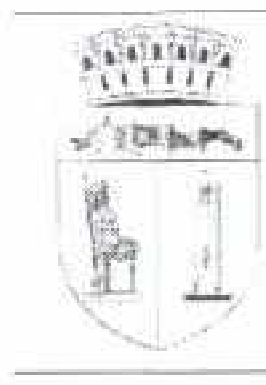
\includegraphics[height=1.5cm]{assets/stema-cluj.png}%
\hspace{0.2cm}%
\raisebox{0.5cm}{\parbox[t]{3.5cm}{\textbf{PRIMĂRIA}\\\textbf{CLUJ-NAPOCA}}}
\end{minipage}%
\begin{minipage}[t]{0.30\textwidth}
\centering
\vspace{0.4cm}

\includegraphics[width=5cm]{assets/barcode-431002.png}
\end{minipage}%
\begin{minipage}[t]{0.30\textwidth}
\raggedleft
\vspace{0.6cm}
Nr. \fillline[3cm] / \fillline[1cm]
\end{minipage}

\vspace{0.3cm}
\hrule
\vspace{0.5cm}

\textbf{Către,}

\vspace{0.3cm}

\hspace{0.5cm}\textbf{Primarul Municipiului Cluj-Napoca}

\vspace{0.5cm}

\begin{center}
\textbf{C E R E R E}\\
\textbf{pentru prelungirea valabilităţii certificatului de urbanism}
\end{center}

\vspace{0.4cm}

\hspace{0.5cm}Subsemnatul \underline{ {{nume_complet}} }, CNP \underline{ {{cnp}} }, cu

domiciliul/sediul în judeţul \fillline[5cm], municipiul/oraşul/comuna \fillline[5cm]

\fillline[3cm], satul \fillline[4cm], sectorul \fillline[1cm], cod poştal \fillline[2cm], str. \fillline[5cm]

nr. \fillline[1.5cm], bl. \fillline[1cm], sc. \fillline[1cm], et. \fillline[1cm], ap. \fillline[1cm], telefon/fax \fillline[4cm], e-mail \fillline[4cm],

în conformitate cu prevederile Legii nr. 50/1991, privind autorizarea executării lucrărilor de construcţii, republicată, cu modificările şi completările ulterioare, solicit:

\vspace{0.4cm}

\begin{center}
\textit{\textbf{prelungirea valabilităţii}}\\
\textbf{Certificatului de urbanism}\\
\textbf{nr. \underline{ {{nr_cu_initial}} } din \underline{ {{data_emitere_cu}} }}
\end{center}

\vspace{0.4cm}

\hspace{0.5cm}pentru imobilul teren şi/sau construcţii, situat în \underline{ {{adresa_imobil}} }

municipiul/oraşul/comuna \fillline[5cm], satul \fillline[5cm],

sectorul \fillline[1cm], cod poştal \fillline[2cm], str. \fillline[5cm] nr. \fillline[1.5cm], bl. \fillline[1cm], sc. \fillline[1cm]

et. \fillline[1cm], ap. \fillline[1cm], sau identificat prin$^{3)}$ \fillline[7cm]

\hrulefill

\vspace{0.4cm}

\hspace{0.5cm}Solicit prelungirea valabilităţii certificatului de urbanism nr. \underline{ {{nr_cu_initial}} } / \underline{ {{data_emitere_cu}} }

din data de \fillline[3cm] până la data de \fillline[3cm]

\vspace{0.3cm}

\textbf{Motivul prelungirii:} \underline{ {{motiv_prelungire}} }

\vfill
\hrule
\vspace{0.2cm}
\small
www.primariaclujnapoca.ro \\
telefon: 0264/596.030 \\
Cluj-Napoca, str. Moţilor, nr. 3 \hfill \textbf{
\includegraphics[width=4cm]{assets/barcode-431002.png}}

\vspace{0.2cm}
\footnotesize
Timp estimativ de completare: 10 minute\\
Datele personale care vă sunt solicitate prin prezenta cerere vor fi prelucrate numai în vederea procesării și soluționării solicitării dumneavoastră. Primăria municipiului Cluj-Napoca garantează securitatea procesării datelor și arhivarea acestora în conformitate cu prevederile legale în vigoare. Responsabilul Primăriei municipiului Cluj-Napoca cu protecția datelor poate fi contactat pe adresa de email dpo@primariaclujnapoca.ro.\\
În conformitate cu Regulamentul nr. 679/2016 aveți dreptul de a solicita Primăriei municipiului Cluj-Napoca, în ceea ce priveşte datele cu caracter personal referitoare la persoana vizată, accesul la acestea, rectificarea sau ştergerea acestora sau restricţionarea prelucrării sau a dreptului de a vă opune prelucrării, precum şi a dreptului la portabilitatea datelor.

\newpage

\noindent
\begin{minipage}[t]{0.40\textwidth}
\vspace{0pt}
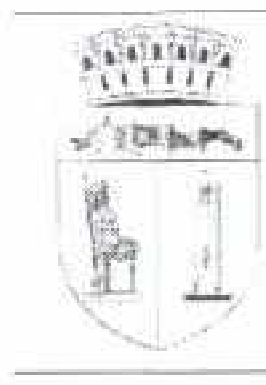
\includegraphics[height=1.5cm]{assets/stema-cluj.png}%
\hspace{0.2cm}%
\raisebox{0.5cm}{\parbox[t]{3.5cm}{\textbf{PRIMĂRIA}\\\textbf{CLUJ-NAPOCA}}}
\end{minipage}%
\begin{minipage}[t]{0.30\textwidth}
\centering
\vspace{0.4cm}

\includegraphics[width=5cm]{assets/barcode-431002.png}
\end{minipage}%
\begin{minipage}[t]{0.30\textwidth}
\raggedleft
\vspace{0.6cm}
Nr. \fillline[3cm] / \fillline[1cm]
\end{minipage}

\vspace{0.3cm}
\hrule
\vspace{0.5cm}

\textit{\textbf{Anexez prezentei cereri:}}$^{1}$
\begin{itemize}[leftmargin=*]
\item certificatul de urbanism nr. \underline{ {{nr_cu_initial}} } / \underline{ {{data_emitere_cu}} } . -- \textbf{în original}
\item documentul privind achitarea taxei (30\% din taxa de emitere a certificatului de urbanism)
\end{itemize}

\vspace{0.5cm}

\checkboxempty\ Prin prezenta solicit comunicarea răspunsului pe următoarea adresă de e-mail:\\
\hrulefill

\vspace{0.3cm}

\checkboxempty\ Mă oblig să comunic instituției orice modificare intervine în legătură cu această adresă de e-mail

\checkboxempty\ Îmi exprim consimțământul ca Primăria Municipiului Cluj-Napoca să comunice orice informații, date personale, clarificări și completări pe adresa de e-mail indicată mai sus

\checkboxempty\ Am luat la cunoștință faptul că în cazul nefuncționării serverului de e-mail comunicat sau în cazul adresei greșite de e-mail, Municipiul Cluj-Napoca nu poate fi tras la răspundere pentru acest lucru

\vspace{1.5cm}

\hfill Semnătura$^{5)}$

\hfill \underline{ {{nume_complet}} }

\vspace{0.5cm}

\hspace{4cm}L.S.

\vspace{0.5cm}

Data \fillline[4cm]

\vspace{0.5cm}

\scriptsize
$^{1}$Primăria municipiului Cluj-Napoca asigură gratuit fotocopierea documentelor.\\
Pentru documentele emise de către alte instituții publice, organe de specialitate ale administrației publice centrale și locale, precum și persoane juridice de drept privat, care potrivit legii au obținut statut de utilitate publică sau sunt autorizate să presteze un serviciu public, în regim de putere publică, pe care solicitantul nu le depune, acesta are posibilitatea de a-și da consimțământul expres ca Primăria municipiului Cluj-Napoca să obțină în numele său copii sau extrase ale acestora.

\vfill
\hrule
\vspace{0.2cm}
\small
www.primariaclujnapoca.ro \\
telefon: 0264/596.030 \\
Cluj-Napoca, str. Moţilor, nr. 3 \hfill \textbf{
\includegraphics[width=4cm]{assets/barcode-431002.png}}

\end{document}
